% Bsp. eines Hauptteils

\chapter{Grundlagen}
\label{sec:grundl}

\section{Funktionsprinzip, Vorteile und Herausforderungen des modernen Cloud Computings}

\subsection{Definition und Funktionsweise}

Das National Institute of Standards and Technology (NIST) der Vereinigten
Staaten von Amerika definiert Cloud Computing im Abstract der NIST SP-800-145
folgendermaßen:\\

Cloud computing is a model for enabling ubiquitous, convenient, on-demand network access to a shared
pool of configurable computing resources (e.g., networks, servers, storage, applications, and services) that
can be rapidly provisioned and released with minimal management effort or service provider interaction.
This cloud model is composed of five essential characteristics, three service models, and four deployment
models.\\

Cloud Computing beschreibt ein Modell das es ermöglicht ortsunabhängig, zweckdienlich und
zeitunabhängig auf einen konfigurierbaren Pool an Computerresourcen (Netzwerke, Server,
Datenspeicher, Anwendungen und Services) zuzugreifen die schnell und mit minimalem
Aufwand und minimaler notwendiger Interaktion bereitgestellt und wieder abgebaut
werden können.
Dieses Cloud Modell beschreibt fünf essentielle Charakteristiken, drei Servicemodelle
und vier Bereitstellungsmodelle.\\

Weiter definiert das Dokument die fünf Charakteristiken in den folgenden Punkten:\\

On-demand-self-service: Der Nutzer kann eigenmächtig die benötigten Resourcen
automatisch bereitstellen, es wird keine menschliche Interaktion benötigt.

Broad network access: Auf Leistungen wird über das normale Internet mit standard
Mechanismen die die Nutzung von Thin Clients und Fat Clients (Smartphones, Tablets,
Laptops oder Workstations) fördern zugegriffen.
 
Resource pooling: Die Computerresourcen des Anbieters werden in einem gemeinsamen Pool
für mehrere Kunden in einem mandantentauglichen Modell bereitgestellt, physische und
virtuelle Resourcen werden nach dynamisch zugewiesen und entsprechend der Nachfrage
neu verteilt. Es wird eine empfundene Ortsunabhängigkeit hergestellt indem der Nutzer
kein genaues Wissen darüber besitzt wo sich dessen Resources befinden, auf höherem
Level wie beispielsweise dem Staat, der Region oder auch Rechenzentrum kann
der Ort vom Nutzer spezifiziert werden. Die bereitgestellten Resourcen beinhalten
zum Beispiel Datenspeicher, Rechenleistung, Rechenspeicher und Netzwerkbandbreite.

Rapid elasticity: Rechenkapazitäten werden dehnbar bereitgestellt und abgebaut,
teilweise automatisch, um entsprechend der Nachfrage schnell hoch- und wieder
zurück skalieren zu können, Rechenkapazitäten erscheinen dadurch unbegrenzt und
zu jeder Zeit in jedem Umfang bereitgestellt werden.

Measured service: Cloud systeme kontrollieren und optimieren Resourcennutzung
automatisch mithilfe eines Messungs-systems dass auf einer abstrakten Ebene den
entsprechenden Service (Datenspeicher, Rechenleistung, Benutzerkonten) überwacht,
kontrolliert und Bericht erstattet um sowohl für Anbieter als auch Kunden Transparenz
herzustellen.\\

Es wird zwischen drei grundlegende Cloud Service Modellen unterschieden: Infrastructure
as a Service (IaaS), Platform as a Service (PaaS) und Software as a Service (SaaS).

\begin{figure}[H]
  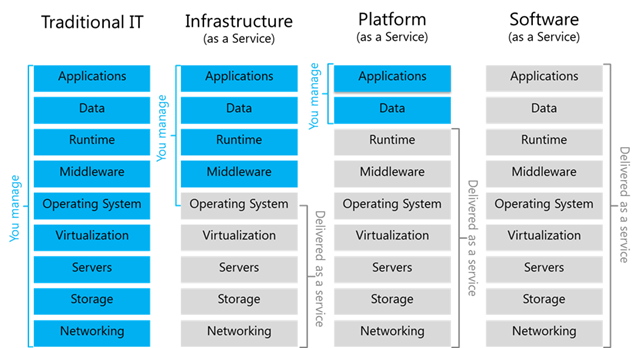
\includegraphics[width=1.0\textwidth]{fig/ch-hauptteil/Service-Models.png}
  \caption{Die grundlegenden Cloud Service Modelle im Überblick}
  \centering
\end{figure}

Infrastructure as a Service: Der Nutzer hat die Fähigkeit Rechenleistung, Datenspeicher
Netzwerke und weitere fundamentale Computerresourcen bereitzustellen und beliebige Software
darauf zu betreiben, dazu können Betriebssysteme und Anwendungen gehören. Die
darunterliegende Infrastruktur wird vom Anbieter betrieben, der Nutzer  kann aber
eingeschränkte Kontrolle über bestimmte Komponenten haben, dazu gehören beispielsweise
Firewalls.

Platform as s Service: Der Nutzer verfügt über die Fähigkeit seine eingkaufte oder
selbst erstellten Anwendungen auf der Cloud Infrastruktur zu betreiben, die notwendige
Umgebung die über Sprachen, Bibliotheken, Tools und Services verfügt wird vom Anbieter
bereitgestellt. Die darunter liegende Infrastruktur mit Netzwerken, Servern,
Betriebssystemen und Speicher wird vom Anbieter betrieben, der Nutzer hat die Kontrolle
über die Anwendung und Konfiguration der Umgebung in der die Anwendung betrieben wird.

Software as a Service: Dem Nutzer wird der Zugriff auf die vom Anbieter in der
Cloud Infrastruktur betriebenen Softwareanwendung gewährt. Auf diese wird mithilfe
eines Thin oder Fat Clients zugegriffen, dabei kümmert sich der Nutzer nicht um den
Betrieb und die Konfiguration der darunterliegenden Cloud Infrastruktur wie
Netzwerke, Server, Betriebssystem, Speicher und die Anwendung selbst mit Ausnahme
eingeschränkter Nutzereinstellungen.

Die von NIST unterschiedenen grundlegenden Service Modellen können noch weiter
differenziert werden.
Ein Beispiel hierfür ist das Modell Function as a Service (FaaS) als subset von PaaS.\\
FaaS erlaubt es Programmcode auszuführen ohne sich um die Bereitstellung weiterer 
Infrastruktur kümmern zu müssen wie es der Betrieb eines gewöhnlichen Microservices
verlangt.\\

In Art der Bereitstellung eines Cloud Services werden vier grundlegende Modelle
unterschieden; Public, Private, Hybrid und Community Cloud Modelle.\\

Private: Die Cloud Infrastruktur wird ausschließlich für die Nutzung durch eine einzige
Organisation mit mehreren Nutzern bereitgestellt. Besitz und Betrieb liegen dabei
entweder bei der selben Organisation, einer Drittpartei oder einer Kombination beider, 
die Infrastruktur kann dabei On- oder Off Premise betrieben werden.

Public: Die Public Cloud steht für die Nutzung durch die allgemeine Öffentlichkeit bereit.
Die Cloud Infrastruktur befindet sich im Besitz eines Unternehmens, Bildungseinrichtung,
Regierungsorganisation oder einer Kombination aus diesen und wird auch von der selben
Organisation On Premise betrieben. 

Community: Eine Community Cloud wird von einer Gemeinschaft von Nutzern mit gemeinsamen
Anliegen eingesetzt. Der Besitz und Betrieb liegen dabei bei einem oder mehreren
Mitgliedern dieser Gemeinschaft, einer Drittpartei und kann Off oder On Premise betrieben
werden.

Hybrid: Die Hybrid Cloud besteht aus einer Kombination der beschriebenen Modelle
(Public, Private und Community). Diese bilden dabei eigene Instanzen die aber durch
standardisierte oder proprietäre Schnittstellen den Transfer von Daten und Anwendungen
zwischen den Instanzen erlauben.

\subsection{Zu erwägende Vor- und Nachteile des Einsatzes von Cloud Computing}

\subsubsection{Vorteile und Treiber der Adoption von Cloud Computing}



-Übertragung von Investitionskosten zu Betriebskosten
-Economies of Scale
-Security
-Resilienz
-Skalierbarkeit
-Agilität
-Zukunftsfähigkeit

\subsubsection{Nachteile und Risiken}

-Netzwerkabhängigkeit
-Vendor Lock-in
-Limitierte Kontrolle
-Security und Privacy
-Technische Probleme
-Kosten

\subsection{Erläuterungen der DevOps Prinzipien und Nutzen im Kontext Cloud-nativer Software Entwicklung}
Agile Entwicklung, CI/CD
Qualität und Schnelle Auslieferung gleichermaßen priorisiert

\subsubsection{Vorteile des Einsatzes von GitOps für Continuous devlivery}
Gitops als Prinzip für Cloud native CD
Verwendung bekannter Tools für Repos und Deployment
Push triggert deployment automatisch

\subsection{Überblick über die wichtigsten public Cloud Service Provider}
Google, AWS, Microsoft
IBM Cloud, Alibaba Cloud
Market share

\section{Was ist Infrastructure as Code?}

\subsection{Warum verwendet man IaC?}

\subsection{Technische Abgrenzung von IaC}

\section{Was ist Terraform?}

\subsection{Warum wird Terraform verwendet?}

\subsection{Terraform Alternativen und ergänzende Tools}

\section{Stand der Technik}

\chapter{Aufbau und Untersuchung}
\label{sec:real}
Beschreibung der HW- und SW-Realisierung

\section{High-level Aufbau der Infrastruktur des Versuchsobjekts}
\label{sec:real-unter}
Beispiel Text

\section{Zu analysiernde Aspekte und Eigenschaften}

\section{Konkreter Aufbau in Microsoft Azure}

\section{Konkreter Aufbau in Amazon AWS}

\section{Konkreter Aufbau in Google Cloud Platform}

\section{Literaturverweise}
\label{sec:real-literatur}

Verweise im Text: \cite{doc:stz} und \cite{doc:gun}.

\chapter{Ergebnisse}
\label{sec:ergeb}

\section{Bewertung Azure}

\section{Bewertung AWS}

\section{Bewertung GCP}

\section{Resultate und Vergleichsmatrix}

\enquote{Neuigkeiten} Messergebnisse
